\begin{figure}	
	\centering
	\includegraphics[width = 0.8 \textwidth]{EIN15 16 km/Angeles}
	\includegraphics[width = 0.8 \textwidth]{EIN15 8 km/Angeles}
	\includegraphics[width = 0.8 \textwidth]{CNRM 16 km/Angeles}
	\includegraphics[width = 0.8 \textwidth]{CNRM 8 km/Angeles}
	\caption{
		A comparison of the simulated data (orange) and observed data (blue) in the city of Angeles for each of the four sensitivity runs.
	}
	\label{fig:appendix-sim-vs-observed-angeles}
\end{figure}

\begin{figure}	
	\centering
	\includegraphics[width = 0.8 \textwidth]{EIN15 16 km/Baguio}
	\includegraphics[width = 0.8 \textwidth]{EIN15 8 km/Baguio}
	\includegraphics[width = 0.8 \textwidth]{CNRM 16 km/Baguio}
	\includegraphics[width = 0.8 \textwidth]{CNRM 8 km/Baguio}
	\caption{
		A comparison of the simulated data (orange) and observed data (blue) in the city of Baguio for each of the four sensitivity runs.
	}
	\label{fig:appendix-sim-vs-observed-baguio}
\end{figure}

\begin{figure}	
	\centering
	\includegraphics[width = 0.8 \textwidth]{EIN15 16 km/Manila}
	\includegraphics[width = 0.8 \textwidth]{EIN15 8 km/Manila}
	\includegraphics[width = 0.8 \textwidth]{CNRM 16 km/Manila}
	\includegraphics[width = 0.8 \textwidth]{CNRM 8 km/Manila}
	\caption{
		A comparison of the simulated data (orange) and observed data (blue) in the city of Manila for each of the four sensitivity runs.
	}
	\label{fig:appendix-sim-vs-observed-manila}
\end{figure}

\begin{figure}	
	\centering
	\includegraphics[width = 0.8 \textwidth]{EIN15 16 km/Olongapo}
	\includegraphics[width = 0.8 \textwidth]{EIN15 8 km/Olongapo}
	\includegraphics[width = 0.8 \textwidth]{CNRM 16 km/Olongapo}
	\includegraphics[width = 0.8 \textwidth]{CNRM 8 km/Olongapo}
	\caption{
		A comparison of the simulated data (orange) and observed data (blue) in the city of Olongapo for each of the four sensitivity runs.
	}
	\label{fig:appendix-sim-vs-observed-olongapo}
\end{figure}

\begin{figure}	
	\centering
	\includegraphics[width = 0.8 \textwidth]{EIN15 16 km/Pasay}
	\includegraphics[width = 0.8 \textwidth]{EIN15 8 km/Pasay}
	\includegraphics[width = 0.8 \textwidth]{CNRM 16 km/Pasay}
	\includegraphics[width = 0.8 \textwidth]{CNRM 8 km/Pasay}
	\caption{
		A comparison of the simulated data (orange) and observed data (blue) in the city of Pasay for each of the four sensitivity runs.
	}
	\label{fig:appendix-sim-vs-observed-pasay}
\end{figure}

\begin{figure}	
	\centering
	\includegraphics[width = 0.8 \textwidth]{EIN15 16 km/Quezon}
	\includegraphics[width = 0.8 \textwidth]{EIN15 8 km/Quezon}
	\includegraphics[width = 0.8 \textwidth]{CNRM 16 km/Quezon}
	\includegraphics[width = 0.8 \textwidth]{CNRM 8 km/Quezon}
	\caption{
		A comparison of the simulated data (orange) and observed data (blue) in the city of Quezon for each of the four sensitivity runs.
	}
	\label{fig:appendix-sim-vs-observed-quezon}
\end{figure}